\chapter{Diseño e implementación} % Main chapter title

\label{Chapter3} % Change X to a consecutive number; for referencing this chapter elsewhere, use \ref{ChapterX}

En este capítulo, se presentan de manera concisa las decisiones de diseño del sistema. 
Se abordan aspectos clave como la adquisición de datos, las técnicas de preprocesamiento 
utilizadas y el diseño del modelo de aprendizaje profundo. 

%----------------------------------------------------------------------------------------
%	ADQUISICION DE DATOS
%----------------------------------------------------------------------------------------
\section{Adquisición de datos}
 
\newcommand{\myhash}{\raisebox{\depth}{\#}}

Para llevar a cabo el presente trabajo, se emplearon datos proporcionados por el servicio 
de cardiología e hipertensión del Hospital Alemán. La figura \ref{fig:adquisicion_datos} 
exhibe un diagrama en bloques que ilustra la etapa de adquisición de datos utilizada. 
Es importante destacar que se utilizaron dos conjuntos de datos diferentes. 

\begin{figure}[H]
	\centering
	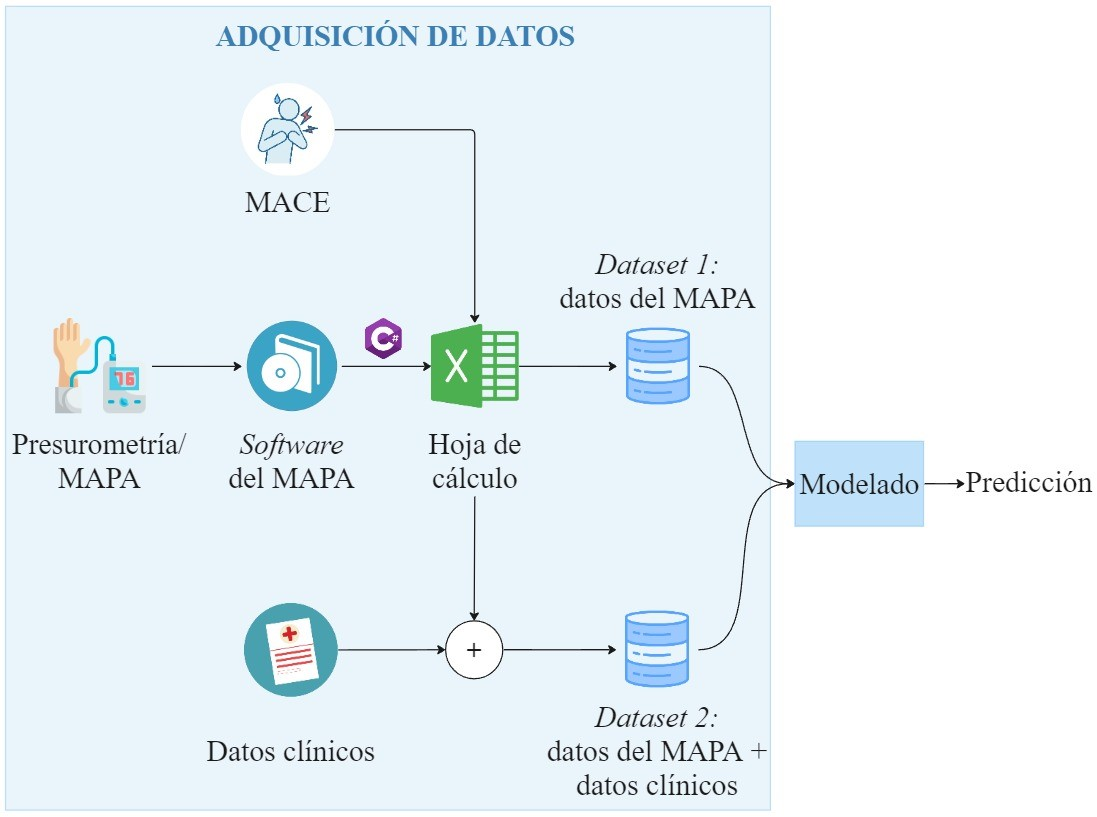
\includegraphics[width=\textwidth]{./Figures/adquisicion_datos2.jpg}
	\caption{Representación esquemática de la etapa de adquisición de datos.}\label{fig:adquisicion_datos}
\end{figure}

El primer \emph{dataset} se compone exclusivamente de información recopilada de las 
presurometrías realizadas a los pacientes hipertensos a partir del año 2013. Luego 
de realizar un MAPA, los datos se almacenan en un \emph{software} especializado de 
los presurómetros. Posteriormente, se extraen utilizando un programa desarrollado 
en C\# para ser registrados en una planilla de cálculo. Sumado a esto, se incluyó 
la variable a predecir (MACE) para cada paciente mediante un análisis exhaustivo 
de su historial clínico. Especificamente, se registró la ocurrencia de 
un accidente cerebrovascular no fatal, infarto agudo de miocardio, insuficiencia 
cardíaca, insuficiencia renal crónica o muerte. En caso de que correspondiera, también 
se incluyó la fecha correspondiente en la que tuvo lugar el evento.

Por otro lado, el segundo conjunto de datos contiene información adicional obtenida 
del historial clínico de cada paciente. Estos datos clínicos se agregan a la misma 
hoja de cálculo mencionada anteriormente, complementando así la información proveniente 
de las presurometrías.

El objetivo de utilizar dos \emph{datasets} es evaluar la calidad de los datos de 
las presurometrías para generar inferencias de manera independiente. En otras palabras, 
se buscó determinar en qué medida los datos del MAPA pueden ser utilizados por sí solos 
para obtener predicciones significativas y precisas de MACE. Al mismo tiempo, se procuró 
evaluar si la incorporación de información clínica contribuye a un mejor desempeño del 
modelo en términos de tasa de falsos negativos, AUC y otras métricas relevantes.


%----------------------------------------------------------------------------------------
% 3.1.1 Descripción del conjunto de datos

\subsection{Descripción del conjunto de datos}

El primer conjunto de datos comprende las variables derivadas del MAPA, junto con 
el valor de MACE y la fecha del evento asociado. A continuación, se brinda una 
descripción detallada de las variables provenientes de las presurometrías: 

\begin{itemize}
  \item Fechaest: corresponde a la fecha en la cual se realizó la presurometría.
  \item PASm24: representa la presión arterial sistólica media durante todo el MAPA.
	\item PADm24: representa la presión arterial diastólica media durante todo el MAPA.
  \item FCm24: representa la frecuencia cardíaca media durante todo el MAPA.
  \item PAMm24: representa la presión arterial media durante todo el MAPA.
  \item PPm24: representa la presión de pulso media durante todo el MAPA.
  \item PASsd24: indica el desvío estándar de la presión arterial sistólica media durante todo el MAPA. 
  \item PADsd24: indica el desvío estándar de la presión arterial diastólica media durante todo el MAPA.
  \item FCsd24:  indica el desvío estándar de la frecuencia cardíaca media durante todo el MAPA.
  \item PAMsd24: indica el desvío estándar de la presión arterial media durante todo el MAPA.
  \item PPsd24: indica el desvío estándar de la presión de pulso media durante todo el MAPA.
  \item PASmDIA: representa la presión arterial sistólica media diurna.
  \item PADmDIA: representa la presión arterial diastólica media diurna.
  \item FCmDIA: representa la frecuencia cardíaca media diurna.
  \item PAMmDIA: representa la presión arterial media diurna.
  \item PPmDIA: representa la presión de pulso media diurna.
  \item htaloadsbpDIA: se refiere al porcentaje de lecturas de la presión arterial sistólica que exceden el valor de referencia de 135 mmHg durante el día.
  \item htaloaddbpDIA: se refiere al porcentaje de lecturas de la presión arterial diastólica que exceden el valor de referencia de 85 mmHg durante el día.
  \item HTAdia01: se utiliza para determinar si un paciente presenta hipertensión diurna (HTAdia01 = 1) o normotensión diurna (HTAdia01 = 0). Se considera hipertensión diurna cuando la presión arterial sistólica es superior a 135 mmHg y la presión arterial diastólica es superior a 85 mmHg durante el día, mientras que se define como normotensión diurna cuando no se cumplen estos criterios.
  \item PASmNOCHE: representa la presión arterial sistólica media nocturna.
  \item PADmNOCHE: representa la presión arterial diastólica media nocturna.
  \item FCmNOCHE: representa la frecuencia cardíaca media nocturna.
	\item PAMmNOCHE: representa la presión arterial media nocturna.
	\item PPmNOCHE: representa la presión de pulso media nocturna.
  \item htaloadsbpNOCHE: representa el porcentaje de lecturas de la presión arterial sistólica que exceden el valor de referencia de 125 mmHg durante la noche.
  \item htaloaddbpNOCHE: se refiere al porcentaje de lecturas de la presión arterial diastólica que exceden el valor de referencia de 70 mmHg durante la noche.
  \item HTAnoche01: se define como hipertensión nocturna (HTAnoche01 = 1) cuando la presión arterial sistólica es superior a 120 mmHg y la presión arterial diastólica es superior a 70 mmHg durante la noche. En caso contrario, se considera normotensión nocturna (HTAnoche01 = 0).
  \item Nondipper01: se utiliza para clasificar a los pacientes en función de la disminución de la presión arterial nocturna. Cuando la presión arterial no disminuye en un 10\% durante la noche, se considera un indicador de alto riesgo cardiovascular y se denominan \emph{non-dippers} (Nondipper01 = 1). Por otro lado, aquellos pacientes cuya presión arterial disminuye en un 10\% durante la noche se denominan \emph{dippers} (Nondipper01 = 0).
\end{itemize}


El segundo conjunto de datos, por su parte, incluye todas las variables mencionadas anteriormente, junto con
9 variables adicionales extraídas del historial clínico de cada paciente. Estas incluyen:

\begin{itemize}
  \item Talla: se refiere a la medida de la longitud del cuerpo de una persona y se expresa en centímetros.
  \item Peso: se refiere a la medida de la masa corporal del paciente expresada en kilogramos.
  \item IMC: el índice de masa corporal (IMC) es una medida utilizada para evaluar la relación entre el peso y la estatura de una persona. Se calcula dividiendo el peso en kilogramos por el cuadrado de la estatura en metros.
  \item Edad: representa el tiempo transcurrido desde el nacimiento de un individuo, medido en años.
  \item Sexo: indica si el paciente es hombre (Sexo = 0) o mujer (Sexo = 1).
  \item DBT: indica la presencia (DBT = 1) o ausencia (DBT = 0) de diabetes en un paciente, una enfermedad metabólica crónica caracterizada por niveles elevados de glucosa en sangre.
  \item Tabaquismo: indica si un paciente tiene adicción a la nicotina (Tabaquismo = 1) o no presenta dicha adicción (Tabaquismo = 0).
  \item Dislipemia: señala la presencia (Dislipemia = 1) o ausencia (Dislipemia = 0) de una alteración en los niveles de lípidos en sangre en un paciente.
  \item HVI: indica la presencia (HVI = 1) o ausencia (HVI = 0) de un engrosamiento de la pared del ventrículo izquierdo como consecuencia de la hipertensión en el paciente.
\end{itemize}

%------------------------------------------------------------------------
%	PREPROCESAMIENTO DE DATOS
%----------------------------------------------------------------------------------------
\section{Preprocesamiento de datos}
En la siguiente sección, se proporciona una descripción detallada del preprocesamiento de datos 
realizado en este trabajo. El objetivo principal de esta etapa fue la obtención de un conjunto de 
datos final de alta calidad y utilidad para su posterior análisis y modelado. En la subsección 
\ref{sec:Conjunto1} se describe el procesamiento realizado al conjunto de datos de presurometrías. 
Posteriormente, en la subsección \ref{sec:Conjunto2} se aborda el procesamiento 
llevado a cabo en el conjunto de datos que combina los datos del MAPA y los datos clínicos.

%------------------------------------------------------------------------
%	datos presurometrias
%%%%%%%%%%%%%%%%%%%%%%%
\subsection{Conjunto de datos de presurometrías}
\label{sec:Conjunto1}

El conjunto de datos utilizado consta de 491 informes del MAPA y se caracteriza por no tener datos faltantes. 
Este \emph{dataset} incluye: 3 variables categóricas (HTA durante el día, HTA durante la noche y \emph{non-dipper}), 
2 variables de fecha (fecha del estudio y fecha de MACE) y 25 variables numéricas continuas.


\subsubsection{Distribuciones de las variables numéricas}
Se realizó un análisis de las distribuciones de los datos con el objetivo de determinar si siguen una distribución 
normal y si existen valores extremos. 

En primer lugar, se llevaron a cabo pruebas visuales utilizando gráficos Q-Q 
(cuantil-cuantil) e histogramas. El gráfico Q-Q es una herramienta utilizada para comparar dos distribuciones de 
probabilidad trazando sus cuantiles uno contra el otro. Aunque no es una prueba estadística formal, proporciona 
una forma sencilla e intuitiva de verificar qué distribución sigue un conjunto de datos. Por otro lado, el 
histograma permite visualizar la distribución de frecuencias de los datos de una variable. 

En la figura \ref{fig:qqplot_a} se representan los gráficos Q-Q de las presiones y la frecuencia cardíaca 
media durante un período de 24 horas. Por su parte, en la figura \ref{fig:qqplot_b} se muestran los 
gráficos Q-Q de las cargas hipertensivas sistólicas y diastólicas durante el día y la noche. Además, en 
las figura \ref{fig:histogram_1} se presentan los histogramas correspondientes a las mismas variables.
Al examinar los gráficos, se observa que las variables PAD, PAM y frecuencia cardíaca (FC) siguen una 
distribución normal, mientras que las variables PAS y PP muestran una ligera sesgadura hacia la derecha. 
Cabe mencionar que las presiones y la FC mantienen la misma distribución tanto durante el día como durante 
la noche, aunque estos gráficos no se muestran en las figuras \ref{fig:qqplot_1} y \ref{fig:histogram_1}.
En cuanto a las cargas hipertensivas sistólicas, se aprecia una distribución asimétrica hacia la derecha, 
mientras que las cargas hipertensivas diastólicas presentan una distribución casi uniforme.

\begin{figure}[H]
	\centering
	\hspace{1em}
	\subcaptionbox{Gráficos Q-Q de la PAS, PAD, FC, PAM y PP durante 24 h.\label{fig:qqplot_a}}
	[0.45\linewidth]{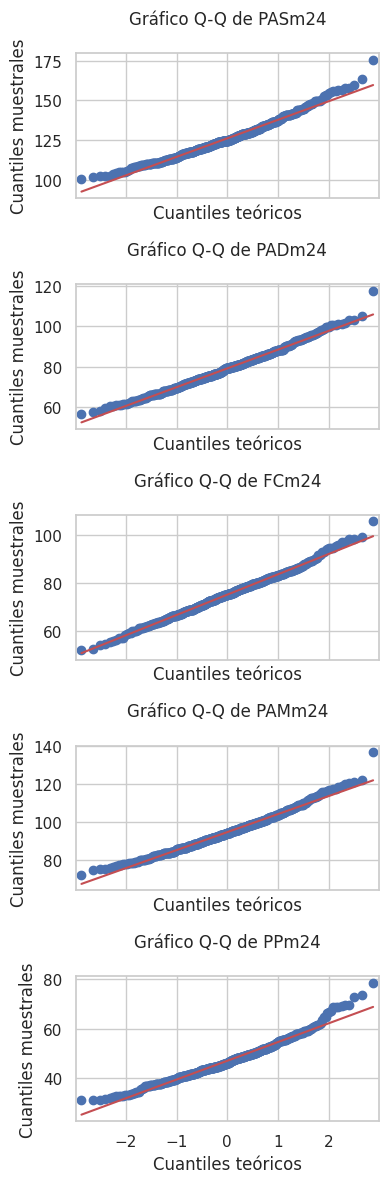
\includegraphics[height=20cm]{./Figures/qqplot_dataset1a.png}}
	\hspace{1em}
	\subcaptionbox{Gráficos Q-Q de las cargas hipertensivas sistólicas y diastólicas \\durante el día y la noche.\label{fig:qqplot_b}}
	[0.45\linewidth]{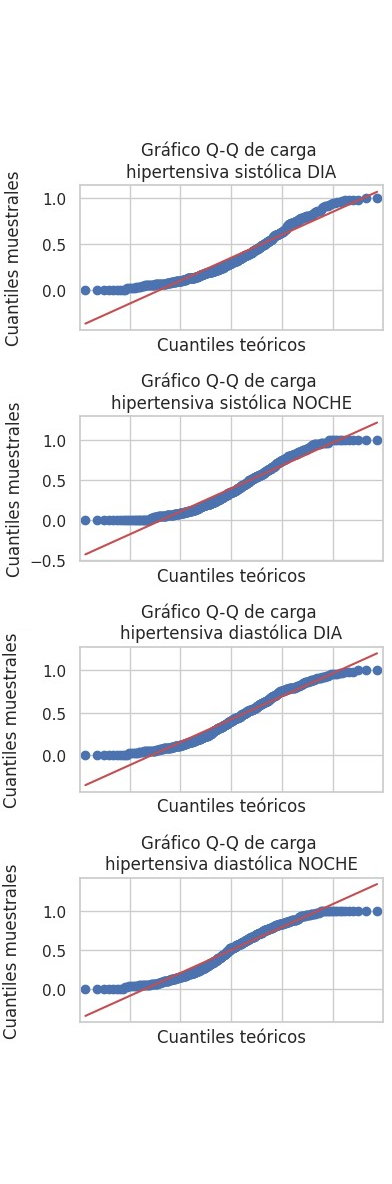
\includegraphics[height=20cm]{./Figures/qqplot_dataset1b.png}}
	\caption{Gráficos Q-Q de variables cuantitativas.}\label{fig:qqplot_1}
\end{figure}

\begin{figure}[H]
	\centering
	\hspace{1em}
	\subcaptionbox{Histogramas de la PAS, PAD, FC, PAM y PP durante 24 h.\label{fig:hist_a}}
	[0.45\linewidth]{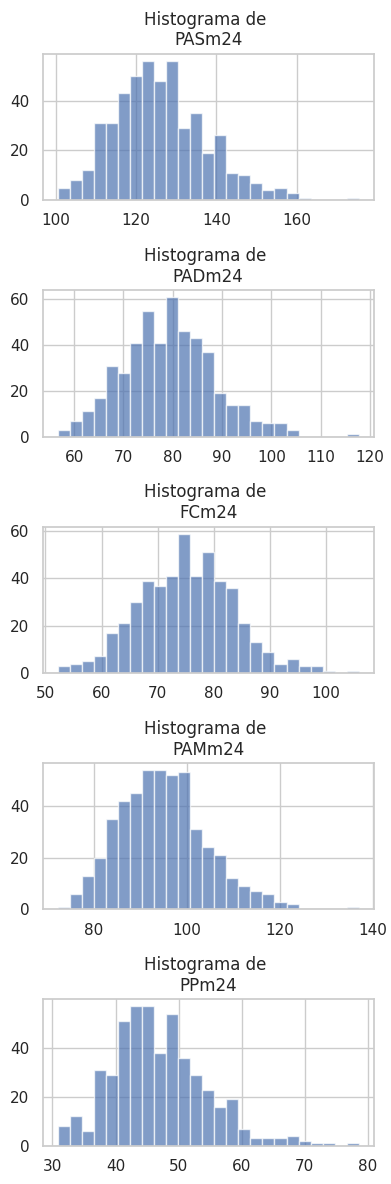
\includegraphics[height=20cm]{./Figures/histograma_dataset1a.png}}
	\hspace{1em}
	\subcaptionbox{Histogramas de las cargas hipertensivas sistólicas y diastólicas durante el día y la noche.\label{fig:hist_b}}
	[0.45\linewidth]{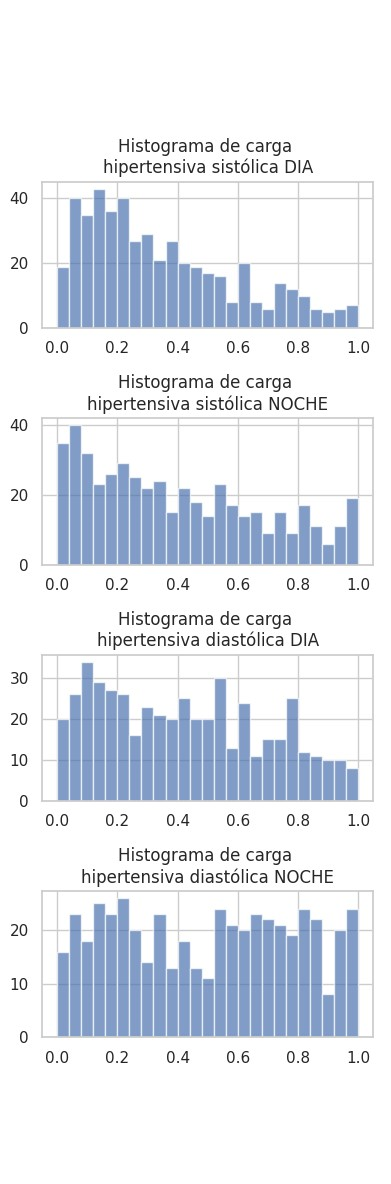
\includegraphics[height=20cm]{./Figures/histograma_dataset1b.png}}
	\caption{Histogramas de variables cuantitativas.}\label{fig:histogram_1}
\end{figure}


%%%%%%%%%%%%%%%%%%%%%%%
%%%%%%%%%%%%%%%%%%%%%%%
%\pagebreak 
%\filbreak 
\subsubsection{Tratamiento de clases desbalanceadas }
En el contexto de este trabajo, se identificó un desbalance de clases, lo cual significa que una de las clases 
está representada por una fracción muy pequeña de las muestras totales. En la figura \ref{fig:desbalance_a} se puede 
observar que solamente un 7.54\% de las muestras pertenecen a la clase positiva, lo que equivale a 37 pacientes con MACE = 1. 
Este desequilibrio en las clases es un fenómeno intrínseco y esperable, ya que refleja la naturaleza del proceso 
que genera los datos. Sin embargo, el desbalance de clases puede crear un sesgo en el modelo de aprendizaje 
automático, ya que tiende a favorecer la predicción de la clase mayoritaria en lugar de capturar adecuadamente 
las instancias de la clase minoritaria. 

Para mitigar este problema, existen diversas técnicas que permiten equilibrar las clases en el conjunto de datos. 
En particular, para este trabajo se empleó la técnica SMOTE, la cual consiste en generar de forma sintética nuevos 
ejemplos de la clase minoritaria. Para lograr un balance más preciso, se combinó el sobremuestreo de la clase 
minoritaria utilizando SMOTE con el submuestreo de la clase mayoritaria mediante el uso de \emph{RandomUnderSampler} \citep{CITE:50}, 
tal como recomienda la publicación científica \emph{"SMOTE: Synthetic Minority Over-sampling Technique"} \citep{CITE:37}.
Esta combinación de técnicas permitió abordar de manera más precisa y equitativa el desafío de la predicción en un escenario 
desbalanceado. El nuevo conjunto de datos balanceado se exhibe en la figura \ref{fig:desbalance_b}.


\begin{figure}[H]
	\centering
	\hspace{1em}
	\subcaptionbox{Conjunto de datos desbalanceado.\label{fig:desbalance_a}}
	[0.45\linewidth]{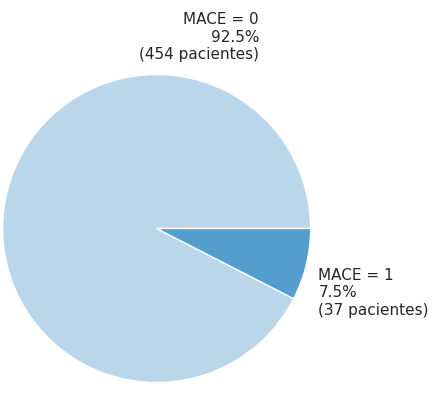
\includegraphics[height=6cm]{./Figures/desbalance_pie.png}}
	\hspace{1em}
	\subcaptionbox{Conjunto de datos después de emplear SMOTE.\label{fig:desbalance_b}}
	[0.45\linewidth]{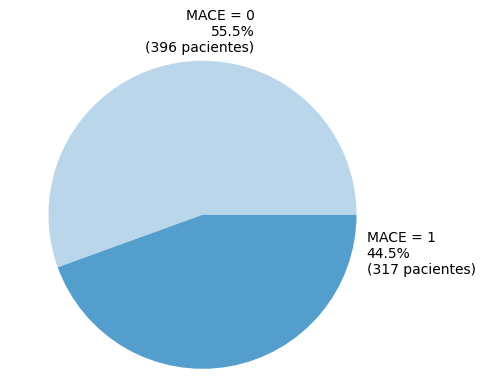
\includegraphics[height=5.5cm]{./Figures/desbalance_smote_under_pie.png}}
	\caption{Conjunto de datos antes y después de aplicar SMOTE y \emph{RandomUnderSampler}.}
\end{figure}

%%%%%%%%%%%%%%%%%%%%%%%
%%%%%%%%%%%%%%%%%%%%%%%
\subsubsection{Normalización de características}
La normalización de los datos es un paso crucial antes de entrenar una red neuronal, y tiene como 
objetivo principal igualar la escala de las características de entrada. Esto es importante puesto 
que las redes neuronales son sensibles a las diferencias de escala entre las variables. En otras 
palabras, cuando los datos presentan diferentes escalas, algunas características con valores numéricos 
más altos pueden tener un impacto desproporcionado en el proceso de entrenamiento. Esto puede ocasionar 
una mayor influencia en los pesos de la red y distorsionar el modelo resultante. 
Además, las funciones de activación utilizadas en las neuronas pueden funcionar de manera óptima 
cuando los datos están normalizados en un rango adecuado.

En este trabajo, se decidió utilizar el método \emph{StandardScaler} de \emph{scikit-learn} \citep{CITE:50} para 
normalizar las características de entrada. Este método aplica una transformación que ajusta la 
media de cada característica a 0 y la desviación estándar a 1. La definición de la transformación 
se muestra en la ecuación \ref{eq:normalizacion}, donde $X$ representa la matriz de características de 
entrada, $\mu$ a la media y $\sigma$ al desvío estándar. 

\begin{equation}
	\label{eq:normalizacion}
	X_{\text{normalizado}} = \frac{X - \mu}{\sigma}
\end{equation}

Al normalizar los datos de esta manera, se garantiza que todas las características tengan la 
misma escala, lo que facilita el proceso de aprendizaje de la red neuronal y mejora la convergencia 
del modelo. En la figura \ref{fig:normalizacion} se muestran a modo de ejemplo las distribuciones de 
la PAS, PAD y FC medias durante 24 horas antes y después de ser normalizadas. 

\begin{figure}[H]
	\centering
	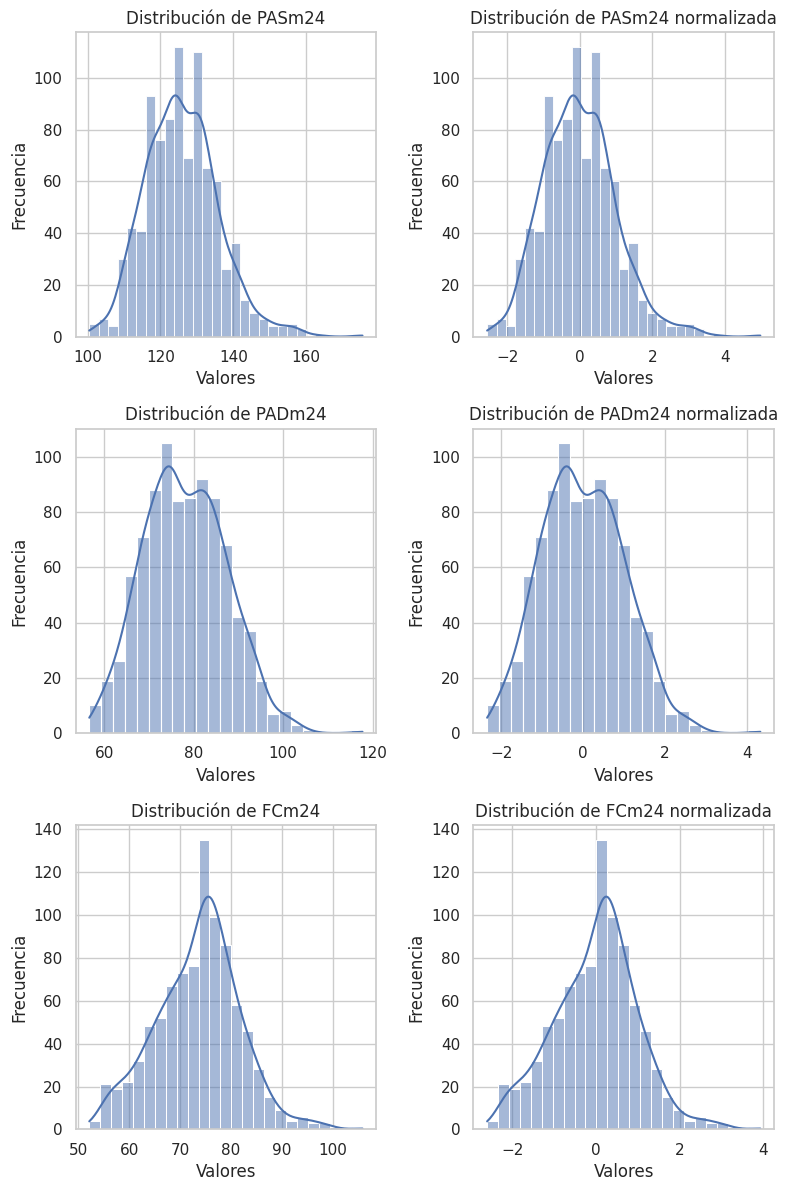
\includegraphics[width=0.8\textwidth]{./Figures/normalizacion.png}
	\caption{Distribuciones de la PAS, PAD y FC durante 24 h \\antes y después de la normalización.}\label{fig:normalizacion}
\end{figure}

%%%%%%%%%%%%%%%%%%%%%%%
%%%%%%%%%%%%%%%%%%%%%%%
\subsubsection{Selección de características}

La selección de variables para un modelo de red neuronal es un proceso crítico que tiene como objetivo 
elegir las variables más relevantes y evitar la inclusión de aquellas que sean redundantes o 
problemáticas. Durante el desarrollo de este trabajo, se identificaron dos variables que son 
combinaciones lineales de otras. Específicamente, se encontró que la presión arterial media y 
la presión de pulso dependen linealmente de la presión arterial sistólica y diastólica. 
Esta relación se definió matemáticamente en la subsección \ref{IntroPresiones} y 
se puede visualizar claramente en la figura \ref{fig:pamypp}. 

\begin{figure}[H]
	\centering
	\hspace{1em}
	\subcaptionbox{Relación lineal de PAM con PAS y PAD.\label{fig:pam}}
	[0.45\linewidth]{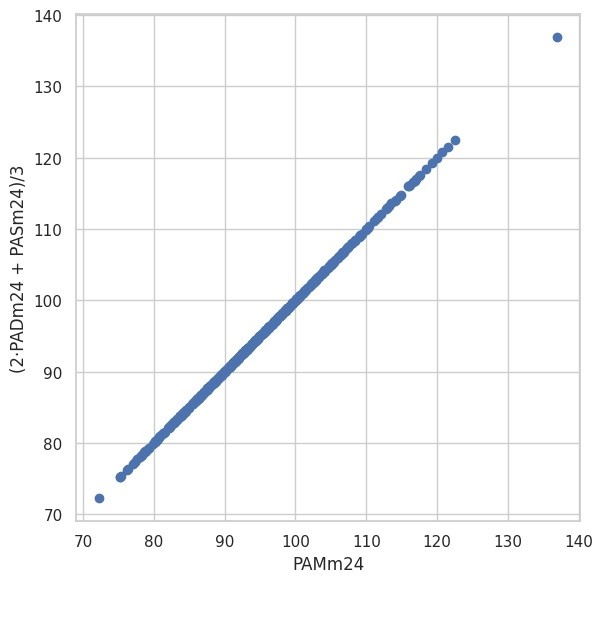
\includegraphics[height=6.5cm]{./Figures/PAM.jpg}}
	\hspace{1em}
	\subcaptionbox{Relación lineal de PP con PAS y PAD.\label{fig:pp}}
	[0.45\linewidth]{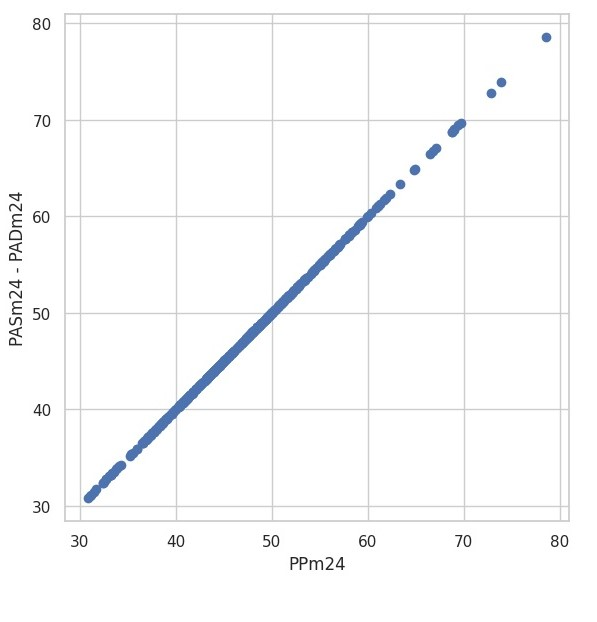
\includegraphics[height=6.5cm]{./Figures/PP.jpg}}
	\caption{Combinaciones lineales de la presión arterial media y presión de pulso con las presiones sistólicas y diastólicas.}\label{fig:pamypp}
\end{figure}


Teniendo en consideración esta información, se tomó la decisión de no incluir estas variables en 
la red neuronal por diversos motivos. En primer lugar, se buscó evitar la redundancia de información. 
Si una variable es una combinación lineal de otras, significa que la información contenida en 
dicha variable ya está presente en las demás. Por lo tanto, su inclusión solo duplicaría la 
información en la red neuronal, lo cual genera una sobrecarga y ralentiza el proceso de 
entrenamiento. Además, es posible que se generen problemas de inestabilidad numérica puesto que incluso 
pequeñas variaciones en los valores de entrada pueden dar lugar a variaciones significativas 
en las salidas. Esto podría comprometer la estabilidad y precisión de la red neuronal, afectando 
negativamente su rendimiento y capacidad de generar resultados confiables. Otro motivo para 
excluir estas variables es evitar que el modelo se ajuste en exceso a los datos de entrenamiento. 
Es posible que esto resulte en una pérdida de generalización, lo que significa que la red tendría 
dificultades para adaptarse a nuevos datos no vistos anteriormente.

En consecuencia, para abordar estos problemas, se decidió eliminar los valores medios y desviaciones 
estándar de PAM y PP. Así, se preservaron únicamente los valores medidos por el presurómetro: la PAS y PAD. 
De este modo, se asegura que la red neuronal se enfoque en las variables fundamentales y se evitan 
los problemas mencionados anteriormente.

Por otro lado, las variables que incluyen fechas son útiles para brindar fiabilidad a 
la base de datos, ya que proporcionan información sobre el momento en el que se realizó el MAPA y, en caso 
de que hubiese ocurrido, el momento en el que se produjo un evento.
Sin embargo, en el contexto de predecir MACE, estas variables pueden considerarse irrelevantes ya 
que no aportan información sustancial para predecir el resultado deseado. En otras palabras, 
la fecha en sí misma no contiene información directa sobre los atributos fisiológicos o clínicos 
que están más relacionados con la ocurrencia de MACE. Además de su falta de 
relevancia, mantener la variable de fecha agregaría una complejidad adicional al modelo 
de red neuronal. La representación y codificación de la fecha como una característica en el 
modelo requiere un procesamiento adicional. Su transformación en valores numéricos o la 
creación de variables categóricas adicionales aumentaría la dimensionalidad de los datos 
y podría dificultar la interpretación de la red neuronal. Por lo tanto, se decidió eliminar 
esta variable con el fin de agilizar el análisis y entrenamiento de la red neuronal. 

Después de realizar el preprocesamiento a la información proveniente del MAPA, el conjunto 
de datos final utilizado para el desarrollo del modelo incluye las siguientes variables de entrada:

\begin{itemize}
	\item PASm24	
  \item PADm24
  \item FCm24
  \item PASsd24 
  \item PADsd24
  \item FCsd24
  \item PASmDIA
  \item PADmDIA
  \item FCmDIA
  \item htaloadsbpDIA 
  \item htaloaddbpDIA   
  \item HTAdia01	
  \item PASmNOCHE
  \item PADmNOCHE
  \item FCmNOCHE
  \item htaloadsbpNOCHE
  \item htaloaddbpNOCHE
  \item HTAnoche01
\end{itemize}


%%%%%%%%%%%%%%%%%%%%%%%%%%%%%%%%%%%%%%%%%%%%%%%%%%%%%%%%%%%%%%%%%%%%%%%%%%%%%%%%%%%%%%%%%%%%
%%%%%%%%%%%%%%%%%%%%%%%%%%%%%%%%%%%%%%%%%%%%%%%%%%%%%%%%%%%%%%%%%%%%%%%%%%%%%%%%%%%%%%%%%%%%
%------------------------------------------------------------------------
%	datos presurometrias + datos clinicos
\subsection{Conjunto de datos de presurometrías y datos clínicos}
\label{sec:Conjunto2}

El segundo conjunto de datos utilizado incorpora los datos clínicos adicionales de los 491 pacientes que 
se realizaron el MAPA, complementando así la información del conjunto de datos anterior. Dado que muchas 
de las variables son las mismas, esta subsección se enfoca exclusivamente en el preprocesamiento aplicado 
a las nuevas variables clínicas. Estas incluyen 4 variables numéricas (talla, peso, IMC y edad) y 5 variables 
categóricas (sexo, diabetes, tabaquismo, dislipemia e hipertrofia ventricular izquierda).


%%%%%%%%%%%%%%%%%%%%%%%
%%%%%%%%%%%%%%%%%%%%%%%
\subsubsection{Distribuciones de las variables numéricas}
Para analizar las variables clínicas numéricas del conjunto de datos, se llevaron a cabo pruebas visuales y 
estadísticas. En la figura \ref{fig:qqplots2} se exhiben los gráficos Q-Q e histogramas para las variables 
de interés. En cuanto a la talla, se observó que los datos siguen una distribución aproximadamente normal. 
Tanto el gráfico Q-Q como el histograma mostraron una forma de campana característica de esta distribución. 
En el caso del peso y el IMC, se encontró una distribución asimétrica positiva. Esto indica que hay una mayor 
concentración de valores más bajos y una dispersión hacia valores más altos. Esto se debe a que la media y la 
mediana del peso fueron de 76 kg, mientras que la moda se situó en 85 kg. Dado que el IMC se calcula a partir 
del peso y la talla, su distribución sigue una tendencia similar a la del peso. Por otro lado, en cuanto a 
la variable de edad, se identificó una distribución asimétrica negativa. Esto sugiere que existe una mayor 
cantidad de personas mayores en el conjunto de datos. La media de la edad fue de 65 años, con una edad mínima 
de 19 años y una máxima de 98 años. La moda de la distribución se encontró en 72 años.

\begin{figure}[H]
	\centering
	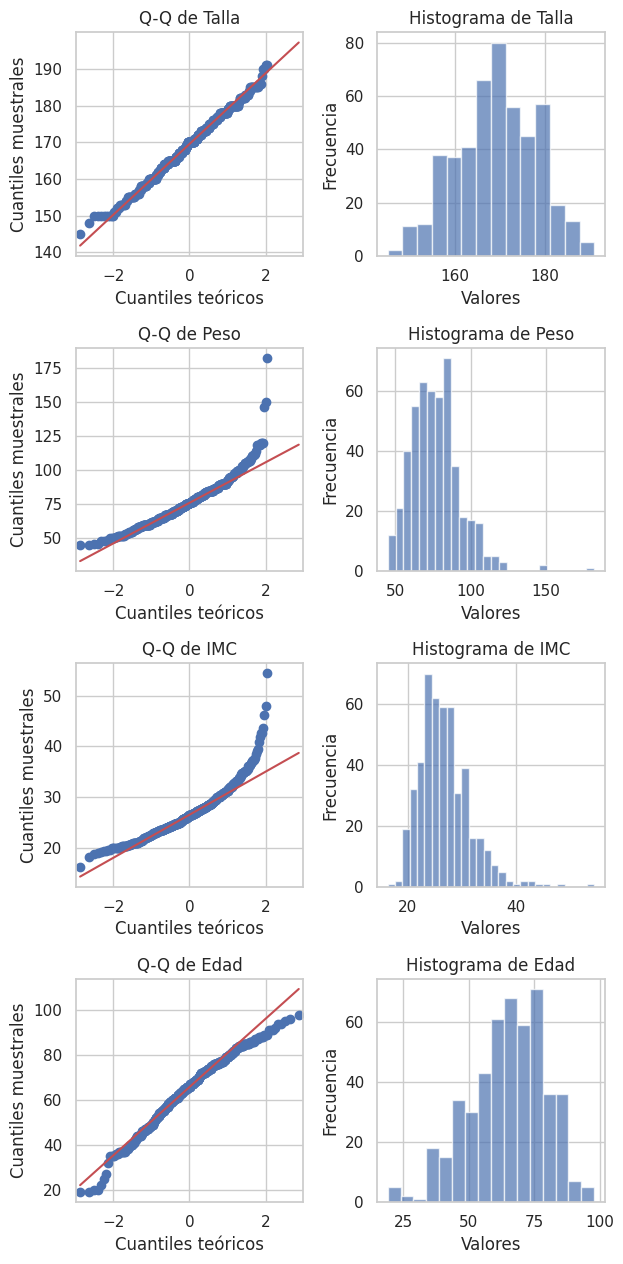
\includegraphics[width=0.8\textwidth]{./Figures/qqplots2.png}
	\caption{Gráficos Q-Q e histogramas de la talla, peso, IMC y edad.}\label{fig:qqplots2}
\end{figure}

Además de los análisis visuales, se realizaron pruebas estadísticas, incluyendo los tests de Shapiro-Wilk 
y Kolmogorov-Smirnov. Los resultados de ambas pruebas indicaron que la talla, el peso y el IMC siguen una 
distribución normal, mientras que la edad no presenta una distribución normal.

%%%%%%%%%%%%%%%%%%%%%%%
%%%%%%%%%%%%%%%%%%%%%%%
%\pagebreak 
\subsubsection{Imputación de valores faltantes}
En el segundo conjunto de datos utilizado, se identificaron diferentes variables con valores faltantes. 
A continuación, se detalla la cantidad de valores ausentes en cada una de estas variables:

\begin{itemize}
  \item Sexo: 1 paciente sin información.
  \item Talla, peso e IMC: 9 pacientes sin datos de talla ni peso, lo cual implica la ausencia del cálculo del IMC.
  \item Dislipemia: 1 paciente sin información.
  \item HVI (hipertrofia ventricular izquierda): 2 pacientes sin información.
\end{itemize}

Ante la presencia de estos valores faltantes, es necesario aplicar técnicas de imputación para completar 
la información y garantizar la integridad de los datos. En este trabajo, se optó por utilizar el método 
\emph{KNNImputer} de \emph{scikit-learn} \citep{CITE:50}. Esta elección se basa en la capacidad del método
para capturar la estructura de los datos y aprovechar la información de las instancias vecinas para la 
imputación. Además, este método es adecuado para manejar variables numéricas y categóricas, lo cual es 
relevante en el contexto de este trabajo.

La imputación de datos faltantes utilizando técnicas como el \emph{KNNImputer} desempeña un papel fundamental 
al minimizar la pérdida de información en conjuntos de datos relativamente pequeños, 
como es el caso de este trabajo. De esta manera, se maximiza la utilidad de los datos disponibles y se evita la exclusión 
de observaciones valiosas debido a la falta de información.

%%%%%%%%%%%%%%%%%%%%%%%
%%%%%%%%%%%%%%%%%%%%%%%

\subsubsection{Tratamiento de clases desbalanceadas}

En relación al tratamiento de desbalance de clases, se aplicó el mismo enfoque que en la subsección 
\ref{sec:Conjunto1} debido a que la variable de salida es la misma. Se utilizó la técnica de sobremuestreo 
SMOTE para abordar el desequilibrio de clases y mejorar la representación de la clase minoritaria en el conjunto de datos. 

%%%%%%%%%%%%%%%%%%%%%%%
%%%%%%%%%%%%%%%%%%%%%%%
\subsubsection{Normalización de características}

Para asegurar que todas las características tengan una escala uniforme, se llevó a cabo un proceso de normalización 
de los datos. Al igual que en la subsección \ref{sec:Conjunto1}, se utilizó el método \emph{StandardScaler} \citep{CITE:50}. La 
figura \ref{fig:normalizacion2} presenta las distribuciones antes y después de la normalización de las variables talla, peso, IMC y edad. Este procedimiento garantiza que todas las variables estén en una escala comparable, 
lo que facilita la interpretación y el análisis de los datos para la red neuronal.

\begin{figure}[H]
	\centering
	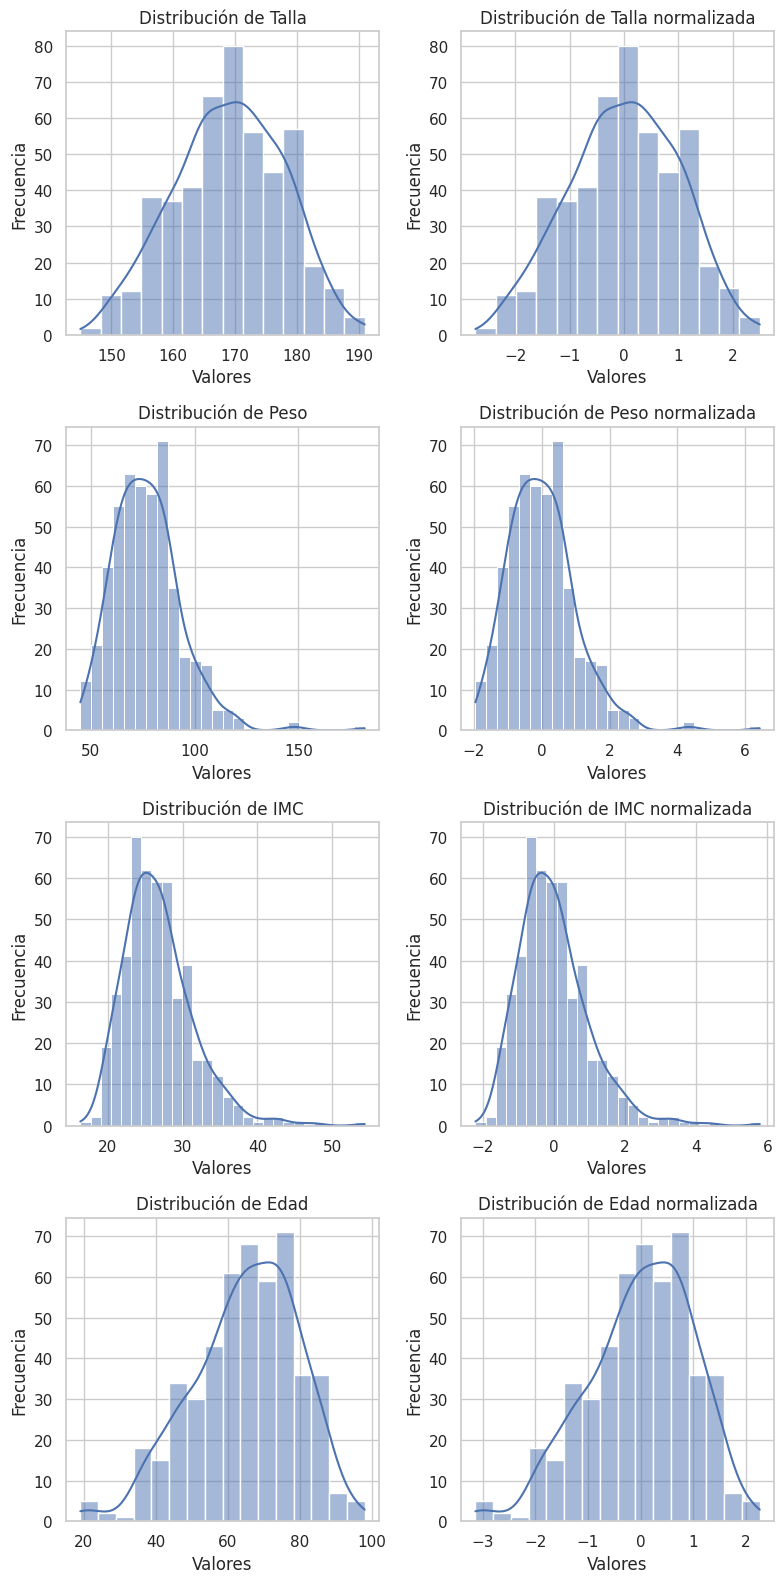
\includegraphics[width=0.7\textwidth]{./Figures/normalizacion2.png}
	\caption{Distribuciones de la talla, peso, IMC y edad antes y después de la normalización.}\label{fig:normalizacion2}
\end{figure}

Después de realizar el preprocesamiento a la información proveniente del MAPA y los datos clínicos, el segundo conjunto de 
datos utilizado para el desarrollo del modelo incluye las siguientes variables de entrada:

\begin{itemize}
  \item PASm24	
  \item PADm24
  \item FCm24
  \item PASsd24 
  \item PADsd24
  \item FCsd24
  \item PASmDIA
  \item PADmDIA
  \item FCmDIA
  \item htaloadsbpDIA 
  \item htaloaddbpDIA   
  \item HTAdia01	
  \item PASmNOCHE
  \item PADmNOCHE
  \item FCmNOCHE
  \item htaloadsbpNOCHE
  \item htaloaddbpNOCHE
  \item HTAnoche01
  \item Talla
  \item Peso
  \item IMC
  \item Edad
  \item Sexo
  \item DBT
  \item Tabaquismo
  \item Dislipemia
  \item HVI
\end{itemize}

%------------------------------------------------------------------------
%	DISEÑO Y DESARROLLO DE MODELOS
%----------------------------------------------------------------------------------------
\section{Diseño y desarrollo de modelos}
El proceso de diseño e implementación de los modelos se llevó a cabo de igual manera para ambos 
conjuntos de datos. A continuación, se presentan en detalle las métricas utilizadas, la 
arquitectura de los modelos y las estrategias implementadas para evitar el \emph{overfitting}.

%%%%%%%%%%%%%%%%%%%%%%%%%%%%%%%%%%%%%%%%%%%%%%%%%%%%%%%%%%%%%%%%%%%%%%%%%%%%%%%%%%%%%%%%%%%%
%%%%%%%%%%%%%%%%%%%%%%%%%%%%%%%%%%%%%%%%%%%%%%%%%%%%%%%%%%%%%%%%%%%%%%%%%%%%%%%%%%%%%%%%%%%%
%------------------------------------------------------------------------
%	Definición de métricas
\subsection{Definición de métricas}

Para evaluar el desempeño de los modelos de forma objetiva, se empleó la métrica AUC. La curva ROC y, 
en particular, el AUC son ampliamente utilizados en la evaluación de modelos de clasificación para 
medir la capacidad de distinguir entre clases positivas y negativas. Para este trabajo en particular, 
la elección se debe a la relevancia clínica de analizar la relación entre la sensibilidad y especificidad. 
En otras palabras, se buscó un equilibrio óptimo entre la detección temprana de casos positivos de MACE 
y la minimización de falsas alarmas. Además, la solicitud específica del cliente de lograr un AUC superior 
al 85\% justificó el uso del AUC como métrica clave. 

A su vez, el servicio de cardiología del Hospital Alemán enfatizó la importancia de evitar falsos negativos. 
Esto implicó que se priorizara la correcta clasificación de casos positivos aunque esto signifique un aumento 
en la tasa de falsos positivos y una posible reducción en otras métricas de evaluación. 

Por otro lado, se calcularon otras métricas además del AUC como \emph{precision}, \emph{recall} y \emph{accuracy} 
para obtener una visión más completa de los resultados del modelo.


%%%%%%%%%%%%%%%%%%%%%%%%%%%%%%%%%%%%%%%%%%%%%%%%%%%%%%%%%%%%%%%%%%%%%%%%%%%%%%%%%%%%%%%%%%%%
%%%%%%%%%%%%%%%%%%%%%%%%%%%%%%%%%%%%%%%%%%%%%%%%%%%%%%%%%%%%%%%%%%%%%%%%%%%%%%%%%%%%%%%%%%%%
%------------------------------------------------------------------------
%	Arquitectura de los modelos
\subsection{Arquitectura de los modelos}
\label{sec:arquitectura}
Una vez definido el objetivo del modelo y preprocesados los datos, se seleccionó la arquitectura básica del modelo. 
Se decidió emplear un perceptrón multicapa puesto que permite capturar relaciones y patrones no lineales en los 
datos. Además, los MLP tienen gran flexibilidad en la representación de características y enorme capacidad para 
aprender representaciones más abstractas y de mayor nivel. De este modo, esta arquitectura puede llevar a una 
mejor habilidad de generalización \citep{CITE:35} \citep{CITE:44}. 

%%%%%%%%%%%%%%%%%%%%%%%
%%%%%%%%%%%%%%%%%%%%%%%
\subsubsection{Definición de la estructura de capas}
Se llevó a cabo una investigación exhaustiva para determinar la configuración óptima del modelo, incluyendo el 
número de capas ocultas y la cantidad de neuronas en cada capa. Dado que no se disponía de conocimientos previos 
sobre la arquitectura ideal, se realizó una búsqueda sistemática de hiperparámetros. Se consideraron diferentes 
alternativas, como 1, 2, 3 o 4 capas ocultas, y se establecieron múltiples opciones para el número de neuronas 
en la primera capa oculta, incluyendo 10, 20, 30, 40 o 50 nodos. En caso de tener múltiples capas ocultas, se 
decidió que la cantidad de neuronas en las capas posteriores fuese la mitad de las de la capa anterior. 
La tabla \ref{tab:tablamodelos} muestra las diferentes combinaciones de modelos que resultaron de esta exploración.


\begin{table}[H]
	\centering
	\caption[Configuraciones de modelos explorados]{Configuraciones de modelos explorados con la cantidad de neuronas por capa oculta.}
	\begin{tabular}{l c c c c}    
		\toprule
		\textbf{Modelo} & \textbf{Capa 1} & \textbf{Capa 2} & \textbf{Capa 3} & \textbf{Capa 4} \\
		\midrule
    \multicolumn{5}{c}{1 capa oculta} \\
    \hline
		1                & 50             & -			          & -               & -	\\
    2                & 40             & -			          & -               & -	\\
    3                & 30             & -			          & -               & -	\\
    4                & 20             & -			          & -               & -	\\
    5                & 10             & -			          & -               & -	\\

    \hline
    \multicolumn{5}{c}{2 capas ocultas} \\
    \hline

    6                & 50             & 25			        & -               & -	\\
    7                & 40             & 20			        & -               & -	\\
    8                & 30             & 15			        & -               & -	\\
    9                & 20             & 10			        & -               & -	\\
    10               & 10             & 5			          & -               & -	\\

    \hline
    \multicolumn{5}{c}{3 capas ocultas} \\
    \hline

    11               & 50             & 25			        & 12              & -	\\
    12               & 40             & 20			        & 10              & -	\\
    13               & 30             & 15			        & 7               & -	\\
    14               & 20             & 10			        & 5               & -	\\
    15               & 10             & 5			          & 2               & -	\\

    \hline
    \multicolumn{5}{c}{4 capas ocultas} \\
    \hline

    16               & 50             & 25			        & 12              & 6	\\
    17               & 40             & 20			        & 10              & 5	\\
    18               & 30             & 15			        & 7               & 3	\\
    19               & 20             & 10			        & 5               & 2	\\
    20               & 10             & 5			          & 2               & 1	\\

		\bottomrule
		\hline
	\end{tabular}
	\label{tab:tablamodelos}
\end{table}

La figura \ref{fig:AUC_exploracion_dataset} muestra los valores promedio de AUC obtenidos 
mediante $k=5$ iteraciones de validación cruzada para los modelos presentados en la tabla \ref{tab:tablamodelos}. 
Se observa que, en el caso del conjunto de datos de presurometrías, los tres modelos con el mejor rendimiento 
en términos de AUC presentan una arquitectura de dos capas ocultas, donde la primera capa cuenta con 30 o más 
nodos (modelos 6, 7 y 8 de la tabla \ref{tab:tablamodelos}). En contraste, para el conjunto de datos que incluye 
información clínica, se encontró que el mejor desempeño en términos de AUC se logró con un modelo de una sola 
capa oculta, con 30 o más nodos en la primera capa (modelos 1, 2 y 3 de la tabla \ref{tab:tablamodelos}).

\begin{figure}[H]
	\centering
	\hspace{1em}
	\subcaptionbox{Valores promedio de AUC obtenidos para el conjunto de datos del MAPA.\label{fig:AUC_exploracion_dataset1}}
	{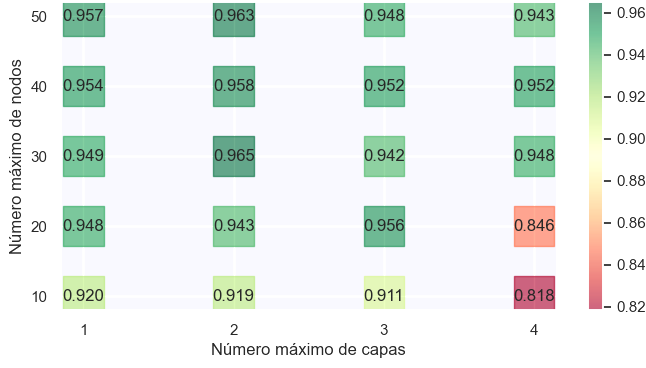
\includegraphics[width=0.96\textwidth]{./Figures/AUC_exploracion_dataset1.png}}
	\hspace{1em}
	\subcaptionbox{Valores promedio de AUC obtenidos para el conjunto de datos del MAPA y datos clínicos.\label{fig:AUC_exploracion_dataset2}}
	{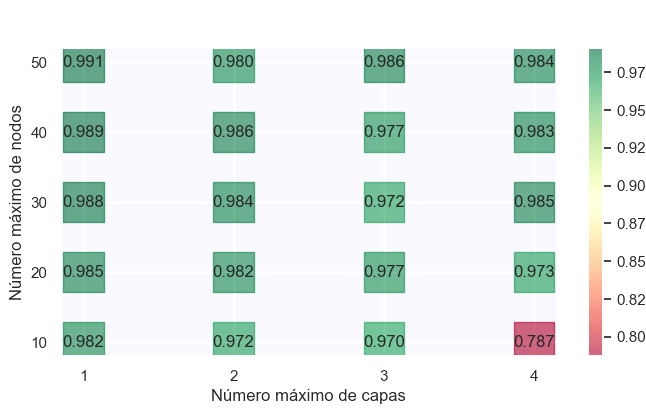
\includegraphics[width=0.96\textwidth]{./Figures/AUC_exploracion_dataset2.png}}
	\caption[Valores promedio de AUC obtenidos mediante $k=5$ iteraciones de validación cruzada.]{Valores promedio de AUC obtenidos mediante $k=5$ iteraciones de validación cruzada para los modelos evaluados.}\label{fig:AUC_exploracion_dataset}
\end{figure}

Con base en los hallazgos anteriores, se llevó a cabo una búsqueda más exhaustiva para determinar la 
arquitectura óptima del modelo. Para el primer conjunto de datos, se realizaron pruebas con modelos 
que incluían dos capas ocultas, explorando diferentes combinaciones. La primera capa se configuró 
con un rango de 20 a 50 nodos, incrementando de uno en uno, mientras que la segunda capa se definió 
con la mitad de las neuronas de la primera capa, es decir, de 10 a 25 nodos, también en incrementos 
de uno. Los resultados obtenidos para cada configuración se registraron en la tabla \ref{tab:tablamodelos_2layers}. 
Por otro lado, para el conjunto de datos que incluye variables clínicas adicionales, se realizó una 
búsqueda de la cantidad de nodos óptima para la única capa oculta, dentro de un rango de 30 a 55, con un 
incremento de un nodo. Los resultados de esta exploración se presentan en la tabla \ref{tab:tablamodelos_1layers}.

\begin{table}[H]
	\centering
	\caption[Configuraciones de modelos explorados para el conjunto de datos del MAPA.]{Configuraciones de modelos explorados con la cantidad de neuronas por capa oculta para el conjunto de datos del MAPA.}
	\begin{tabular}{c c c c c c}    
		\toprule
		\textbf{Capa 1} & \textbf{Capa 2} & \textbf{\emph{Accuracy}} & \textbf{\emph{Precision}} & \textbf{\emph{Recall}}  & \textbf{AUC}\\
		\midrule
    
       50 & 25	& 0.935 $\pm$ 0.021 & 0.902  $\pm$ 0.037	& 0.977  $\pm$ 0.014 & 0.968  $\pm$ 0.016\\
       49 & 24 & 0.930 $\pm$ 0.026 & 0.900  $\pm$ 0.044 & 0.971  $\pm$ 0.005 & 0.964 $\pm$ 0.010\\
       48 & 24 & 0.931 $\pm$ 0.022 & 0.901 $\pm$ 0.033 & 0.971 $\pm$ 0.011 & 0.967 $\pm$ 0.009\\
       47 & 23 & 0.924 $\pm$ 0.017 & 0.890 $\pm$ 0.028 & 0.971 $\pm$ 0.015 & 0.963 $\pm$ 0.008\\
       46 & 23 & 0.922 $\pm$ 0.025 & 0.888 $\pm$ 0.040 & 0.968 $\pm$ 0.011 & 0.953 $\pm$ 0.011\\
       45 & 22 & 0.924 $\pm$ 0.024 & 0.889 $\pm$ 0.041 & 0.973 $\pm$ 0.009 & 0.961 $\pm$ 0.011\\ 
       44 & 22 & 0.921 $\pm$ 0.019 & 0.877 $\pm$ 0.034 & 0.982 $\pm$ 0.015 & 0.958 $\pm$ 0.016\\ 
       43 & 21 & 0.933 $\pm$ 0.017 & 0.902 $\pm$ 0.025 & 0.973 $\pm$ 0.009 & 0.963 $\pm$ 0.012\\ 
       42 & 21 & 0.922 $\pm$ 0.015 & 0.887 $\pm$ 0.021 & 0.968 $\pm$ 0.004 & 0.962 $\pm$ 0.010\\ 
       41 & 20 & 0.920 $\pm$ 0.021 & 0.881 $\pm$ 0.034 & 0.973 $\pm$ 0.011 & 0.961 $\pm$ 0.011\\ 
       40 & 20 & 0.920 $\pm$ 0.028 & 0.880 $\pm$ 0.049 & 0.977 $\pm$ 0.014 & 0.958 $\pm$ 0.017\\ 
       39 & 19 & 0.923 $\pm$ 0.024 & 0.891 $\pm$ 0.033 & 0.966 $\pm$ 0.014 & 0.961 $\pm$ 0.015\\ 
       38 & 19 & 0.923 $\pm$ 0.022 & 0.888 $\pm$ 0.036 & 0.971 $\pm$ 0.011 & 0.956 $\pm$ 0.009\\ 
       37 & 18 & 0.929 $\pm$ 0.012 & 0.898 $\pm$ 0.024 & 0.968 $\pm$ 0.013 & 0.964 $\pm$ 0.012\\ 
       36 & 18 & 0.928 $\pm$ 0.016 & 0.899 $\pm$ 0.032 & 0.966 $\pm$ 0.012 & 0.960 $\pm$ 0.006\\ 
       35 & 17 & 0.925 $\pm$ 0.023 & 0.899 $\pm$ 0.041 & 0.962 $\pm$ 0.006 & 0.960 $\pm$ 0.012\\ 
       34 & 17 & 0.910 $\pm$ 0.008 & 0.866 $\pm$ 0.018 & 0.971 $\pm$ 0.017 & 0.940 $\pm$ 0.011\\ 
       33 & 16 & 0.920 $\pm$ 0.014 & 0.885 $\pm$ 0.022 & 0.966 $\pm$ 0.007 & 0.965 $\pm$ 0.013\\ 
       32 & 16 & 0.921 $\pm$ 0.012 & 0.885 $\pm$ 0.021 & 0.968 $\pm$ 0.013 & 0.959 $\pm$ 0.011\\ 
       31 & 15 & 0.920 $\pm$ 0.020 & 0.881 $\pm$ 0.030 & 0.973 $\pm$ 0.013 & 0.959 $\pm$ 0.009\\ 
       30 & 15 & 0.921 $\pm$ 0.017 & 0.889 $\pm$ 0.028 & 0.964 $\pm$ 0.011 & 0.959 $\pm$ 0.012\\ 
       29 & 14 & 0.923 $\pm$ 0.020 & 0.891 $\pm$ 0.031 & 0.966 $\pm$ 0.007 & 0.961 $\pm$ 0.016\\ 
       28 & 14 & 0.930 $\pm$ 0.034 & 0.901 $\pm$ 0.053 & 0.971 $\pm$ 0.014 & 0.965 $\pm$ 0.021\\ 
       27 & 13 & 0.920 $\pm$ 0.027 & 0.887 $\pm$ 0.046 & 0.966 $\pm$ 0.016 & 0.957 $\pm$ 0.012\\ 
       26 & 13 & 0.909 $\pm$ 0.023 & 0.868 $\pm$ 0.037 & 0.966 $\pm$ 0.016 & 0.953 $\pm$ 0.019\\ 
       25 & 12 & 0.922 $\pm$ 0.014 & 0.887 $\pm$ 0.025 & 0.969 $\pm$ 0.027 & 0.957 $\pm$ 0.012\\ 
       24 & 12 & 0.916 $\pm$ 0.013 & 0.878 $\pm$ 0.021 & 0.968 $\pm$ 0.008 & 0.952 $\pm$ 0.010\\ 
       23 & 11 & 0.919 $\pm$ 0.017 & 0.884 $\pm$ 0.028 & 0.966 $\pm$ 0.012 & 0.950 $\pm$ 0.015\\ 
       22 & 11 & 0.920 $\pm$ 0.019 & 0.885 $\pm$ 0.027 & 0.966 $\pm$ 0.007 & 0.953 $\pm$ 0.013\\ 
       21 & 10 & 0.916 $\pm$ 0.011 & 0.878 $\pm$ 0.022 & 0.968 $\pm$ 0.013 & 0.954 $\pm$ 0.013\\ 
       20 & 10 & 0.920 $\pm$ 0.023 & 0.884 $\pm$ 0.035 & 0.968 $\pm$ 0.017 & 0.945 $\pm$ 0.026\\
      
		\bottomrule
		\hline
	\end{tabular}
	\label{tab:tablamodelos_2layers}
\end{table}


\begin{table}[H]
	\centering
	\caption[Configuraciones de modelos explorados para el conjunto de datos del MAPA y datos clínicos.]{Configuraciones de modelos explorados con la cantidad de neuronas en la capa oculta para el conjunto de datos del MAPA y datos clínicos.}
	\begin{tabular}{l c c c c c c}    
		\toprule
		\textbf{Capa 1} & \textbf{\emph{Accuracy}} & \textbf{\emph{Precision}} & \textbf{\emph{Recall}}  & \textbf{AUC}\\
		\midrule
    
      50 & 0.896 $\pm$ 0.029 & 0.851 $\pm$ 0.032	& 0.931 $\pm$ 0.048 & 0.960  $\pm$ 0.016\\
      49 & 0.909 $\pm$ 0.045 & 0.864 $\pm$ 0.052	& 0.947 $\pm$ 0.050 & 0.963  $\pm$ 0.021\\
      48 & 0.868 $\pm$ 0.014 & 0.839 $\pm$ 0.031	& 0.874 $\pm$ 0.028 & 0.942  $\pm$ 0.023\\
      47 & 0.913 $\pm$ 0.025 & 0.877 $\pm$ 0.026	& 0.937 $\pm$ 0.048 & 0.963  $\pm$ 0.020\\
      46 & 0.878 $\pm$ 0.036 & 0.836 $\pm$ 0.047	& 0.905 $\pm$ 0.045 & 0.953  $\pm$ 0.020\\
      45 & 0.921 $\pm$ 0.028 & 0.879 $\pm$ 0.032	& 0.956 $\pm$ 0.036 & 0.968  $\pm$ 0.007\\
      44 & 0.952 $\pm$ 0.013 & 0.911 $\pm$ 0.024	& 0.991 $\pm$ 0.002 & 0.977  $\pm$ 0.014\\      
      43 & 0.950 $\pm$ 0.019 & 0.899 $\pm$ 0.033	& 0.990 $\pm$ 0.010 & 0.985  $\pm$ 0.005\\
      42 & 0.961 $\pm$ 0.023 & 0.924 $\pm$ 0.034	& 0.994 $\pm$ 0.003 & 0.982  $\pm$ 0.005\\
      41 & 0.956 $\pm$ 0.026 & 0.915 $\pm$ 0.044	& 0.997 $\pm$ 0.003 & 0.985  $\pm$ 0.003\\
      40 & 0.971 $\pm$ 0.016 & 0.939 $\pm$ 0.032	& 0.991 $\pm$ 0.004 & 0.990  $\pm$ 0.007\\
      39 & 0.935 $\pm$ 0.039 & 0.897 $\pm$ 0.034	& 0.966 $\pm$ 0.016 & 0.974  $\pm$ 0.018\\
      38 & 0.943 $\pm$ 0.012 & 0.897 $\pm$ 0.014	& 0.984 $\pm$ 0.011 & 0.979  $\pm$ 0.005\\
      37 & 0.939 $\pm$ 0.036 & 0.900 $\pm$ 0.033	& 0.969 $\pm$ 0.006 & 0.974  $\pm$ 0.013\\
      36 & 0.931 $\pm$ 0.037 & 0.887 $\pm$ 0.035	& 0.969 $\pm$ 0.025 & 0.973  $\pm$ 0.013\\
      35 & 0.889 $\pm$ 0.039 & 0.846 $\pm$ 0.037	& 0.918 $\pm$ 0.062 & 0.952  $\pm$ 0.023\\
      34 & 0.900 $\pm$ 0.031 & 0.847 $\pm$ 0.039	& 0.950 $\pm$ 0.033 & 0.953  $\pm$ 0.023\\
      33 & 0.860 $\pm$ 0.042 & 0.821 $\pm$ 0.054	& 0.880 $\pm$ 0.068 & 0.945  $\pm$ 0.022\\
      32 & 0.871 $\pm$ 0.034 & 0.824 $\pm$ 0.048	& 0.901 $\pm$ 0.076 & 0.944  $\pm$ 0.023\\
      31 & 0.909 $\pm$ 0.048 & 0.869 $\pm$ 0.032	& 0.934 $\pm$ 0.037 & 0.958  $\pm$ 0.024\\
      30 & 0.909 $\pm$ 0.048 & 0.869 $\pm$ 0.032	& 0.934 $\pm$ 0.037 & 0.958  $\pm$ 0.024\\

		\bottomrule
		\hline
	\end{tabular}
	\label{tab:tablamodelos_1layers}
\end{table}

%%%%%%%%%%%%%%%%%%%%%%%%%%%%%%%%%%%%%%%%%%%%
%%%%%%%%%%%%%%%%%%%%%%%%%%%%%%%%%%%%%%%%%%%%
%% AGREGAR!
%%%%FALTA AGREGAR LA TABLA DEL DATASET 2%%%%
%%%%%%%%%%%%%%%%%%%%%%%%%%%%%%%%%%%%%%%%%%%%
%%%%%%%%%%%%%%%%%%%%%%%%%%%%%%%%%%%%%%%%%%%

La figura \ref{fig:arquitectura_datasets} muestra la arquitectura final utilizada para cada conjunto de datos. 
Se observa que se optó por una estructura basada en capas densas, también conocidas como capas 
completamente conectadas, complementadas con capas de \emph{dropout}. La incorporación de las capas 
densas permitió capturar relaciones complejas presentes en los datos, mientras que las capas de 
\emph{dropout} desempeñaron un papel fundamental en la regularización del modelo y en la prevención 
del sobreajuste. Como resultado, se logró obtener un modelo con una mayor capacidad de generalización 
y un mejor desempeño en la predicción de datos desconocidos.


\begin{figure}[H]
	\centering
	\hspace{1em}
	\subcaptionbox{Arquitectura del modelo para el \\conjunto de datos del MAPA.\label{fig:arquitectura_dataset1}}
	{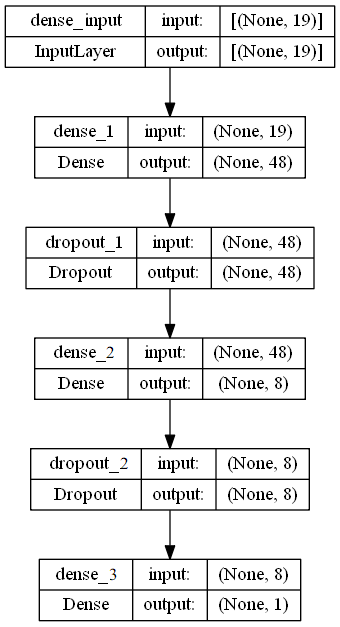
\includegraphics[width=0.45\textwidth]{./Figures/arquitectura_dataset1.png}}
	\hspace{1em}
	\subcaptionbox{Arquitectura del modelo para el conjunto de datos del MAPA y datos clínicos.\label{fig:arquitectura_dataset2}}
	{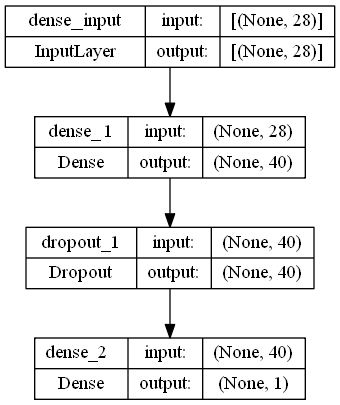
\includegraphics[width=0.45\textwidth]{./Figures/arquitectura_dataset2.png}}
	\caption{Arquitectura elegida para los modelos.}\label{fig:arquitectura_datasets}
\end{figure}

%%%%%%%%%%%%%%%%%%%%%%%
%%%%%%%%%%%%%%%%%%%%%%%
\subsubsection{Selección de funciones de activación, función de pérdida y algoritmo de optimización}
Se empleó la función de activación ReLU en las capas ocultas de la red neuronal. Esta función es 
comúnmente elegida debido a su capacidad para introducir no linealidad en el modelo y capturar 
patrones complejos en los datos. Además, se utilizó la función de activación sigmoide en la capa 
de salida, ya que el problema abordado se trata de una clasificación binaria. La función sigmoide
 es adecuada en este contexto, considerando que mapea los valores de salida a un rango entre 0 y 1, 
 lo que se interpreta como la probabilidad de pertenecer a una de las dos clases posibles.

 Por otro lado, se optó por utilizar la función de pérdida \emph{binary cross entropy} debido a 
 que el problema en cuestión involucra una clasificación binaria. Esta función de pérdida es 
 adecuada para este tipo de problemas, ya que penaliza de manera efectiva las discrepancias 
 entre las predicciones del modelo y los valores reales. En cuanto al algoritmo de optimización, 
 se eligió Adam debido a su eficiencia en la convergencia y adaptabilidad a diferentes tasas de 
 aprendizaje, cómo se explicó en la subsección \ref{sec:optimizador}.

%%%%%%%%%%%%%%%%%%%%%%%
%%%%%%%%%%%%%%%%%%%%%%%
\subsubsection{Ajuste de hiperparámetros}

Una vez definida la arquitectura inicial de la red neuronal, se realizó una búsqueda de hiperparámetros 
adicionales utilizando el enfoque de búsqueda aleatoria, también conocido cómo \emph{RandomSearch} \citep{CITE:50}. 
Esto se combinó con una validación cruzada de $k=5$ iteraciones para evaluar el rendimiento del modelo en diferentes 
conjuntos de datos y asegurar que los hiperparámetros ajustados generalicen bien. Este ajuste tuvo como objetivo 
encontrar el equilibrio adecuado entre el rendimiento del modelo y la capacidad de generalización. 
La tabla \ref{tab:Tabla1} muestra los hiperparámetros que fueron ajustados y sus mejores valores 
para cada conjuntos de datos.

\begin{table}[H]
	\centering
	\caption{Hiperparámetros elegidos para el \emph{dataset} 1 (datos del MAPA) y \emph{dataset} 2 (datos del MAPA y datos clinicos).}
	\begin{tabular}{l c c}    
		\toprule
		\textbf{Hiperparámetros} 	      & \textbf{Valor elegido \emph{dataset} 1} 	& \textbf{Valor elegido \emph{dataset} 2}  \\
		\midrule
    Tasa de aprendizaje            & $1e-03$                   & $1e-2$\\		
    Adam $\epsilon$                   & $1e-08$                 & $1e-7$\\	
    Adam $\beta_1$                   & $0.9$                 & $0.9$\\	
    Adam $\beta_2$                   & $0.999$                 & $0.999$\\		
    Épocas                  & $300$                 & $250$\\	
    Tamaño de lote                  & $32$                 & $32$\\		
    Porcentaje de \emph{dropout}                 & $20\%$                 & $50\%$\\	

		\bottomrule
		\hline
	\end{tabular}
	\label{tab:Tabla1}
\end{table}


%%%%%%%%%%%%%%%%%%%%%%%%%%%%%%%%%%%%%%%%%%%%%%%%%%%%%%%%%%%%%%%%%%%%%%%%%%%%%%%%%%%%%%%%%%%%
%%%%%%%%%%%%%%%%%%%%%%%%%%%%%%%%%%%%%%%%%%%%%%%%%%%%%%%%%%%%%%%%%%%%%%%%%%%%%%%%%%%%%%%%%%%%
%------------------------------------------------------------------------
%	Estrategias implementadas para evitar el \emph{overfitting}
\subsection{Estrategias implementadas para evitar el \emph{overfitting}}
El \emph{overfitting} es un fenómeno que se refiere a la situación en la cual un modelo 
se ajusta excesivamente a los datos de entrenamiento y pierde su capacidad de generalización 
en datos no vistos. En el contexto de este trabajo, se adoptaron varias estrategias 
con el objetivo de mitigar el \emph{overfitting} y garantizar la robustez de los modelos.

En primer lugar, se buscó priorizar la selección 
de modelos más simples, evitando la incorporación de una complejidad excesiva. Esto implicó 
mantener reducido el número de capas y/o neuronas en cada capa del modelo, con el objetivo de 
lograr un equilibrio entre la capacidad de aprendizaje y la generalización.
Además, cómo se mencionó en la subsección \ref{sec:arquitectura}, se incorporaron capas 
de \emph{dropout} en el modelo. Esta técnica consistió en apagar de forma aleatoria un 
porcentaje de las neuronas durante el entrenamiento, para evitar que se ajusten excesivamente 
a los datos de entrenamiento. Al no ser entrenadas, estas neuronas contribuyen a la 
regularización del modelo y ayudan a prevenir el overfitting.
Asimismo, otra estrategia empleada fue el uso de \emph{early stopping}. Esta técnica implica detener 
el proceso de entrenamiento del modelo en el momento en que se observa un aumento en el valor 
del error de validación. De este modo, se buscó evitar el ajuste excesivo y lograr un modelo 
con una precisión óptima en datos no utilizados durante el entrenamiento \citep{CITE:44}.
